\documentclass[conference]{IEEEtran}
\IEEEoverridecommandlockouts
% The preceding line is only needed to identify funding in the first footnote. If that is unneeded, please comment it out.
%\usepackage{cite} Incompatible with biblatex
\usepackage{amsmath,amssymb,amsfonts}
\usepackage{algorithmic}
\usepackage{graphicx}
\usepackage{textcomp} 
\usepackage{hyperref}
\usepackage{xcolor}
\usepackage[style=ieee]{biblatex}
\usepackage[toc,page]{appendix}
\addbibresource{references.bib}
\def\BibTeX{{\rm B\kern-.05em{\sc i\kern-.025em b}\kern-.08em
    T\kern-.1667em\lower.7ex\hbox{E}\kern-.125emX}}

\begin{document}

\title{Which requirements favour which implementation? \\}

\maketitle

\begin{abstract}
This paper will dive in four different implementation of the Insertion Sort algorithm. The four implementations are FSMD (Finite State Machine with Data path), ASIP (Application-Specific Instruction-set Processor), C (software-based implementation) and Custom IP (hardware-based implementation). The implementation will be described in the first part. The second part will look further and focus on the question which requirements favour which implementation. Here different requirements will be presented and evaluated. In the end we present in which situation developing and deploying of a certain implementation makes most sense. 
\end{abstract}

\section{Introduction}

\section{Insertion Sort}
We decided to implement the Insertion Sort Algorithm for the project asignment. It is a well-known and simple sorting algorithm. The concept of Insertion Sort is akin to organizing playing cards in your hand: you divide the cards into two groups, the sorted and the unsorted. Then, you select a card from the unsorted group and insert it into the correct position in the sorted group~\cite{g4g}.\\
It is maily used for small or nearly sorted lists. For a nearly sorted list, the time complexity of Insertion Sort is a $O(n)$ which is the best case. The average and worst case have both a time complexity of $O(n^2)$. Other sorting algorithms such as Merge Sort and Quick Sort are more commonly used due to their lower average time complexities.\\
Insertion Sort is a in-place sorting algotithm which means that its space complexity is at $O(n)$. It needs the same amount of space as the input and only a fixed number of extra inputs.

\section{Implementations}
This section will focus on our four different implementations of the Insertion Sort algorithm. We implemented them in the order in which they are listed in the following sections. We wanted to start with a hardware implementation as we did not feel comfortable enough to start with the ASIP implementation. Therefore we decided to start with the FSMD implementation. This choice turned out to be helpful for both the ASIP and IP Block implementations. For the ASIP, we used the ASMD diagram from our FSMD implementation. Later during the creation of our custom IP block, we started by using the same code which we used in our C-program. \\
The whole group worked together on each implementation, and we completed them one at a time. We made sure the current implementation was fully working before starting the next one. This lead to the work being non-ambigous and the entire group was on the same page during the whole project.

\subsection{FSMD}\label{section:fsmd}
Our implementation started with designing a finite state machine with data path (FSMD) diagram as well as an algorithm state machine with datapath (ASMD) diagram before we started the implementation. We kicked this implementation off by designing the FSMD. There, we chose the parts that were needed such as a RAM, receiving unit and transmission unit as well as comparators and registers. Based on this we defined our data path in accordance to our components. In order to keep the implementation simple and close to the concept, we avoided sending any data to the control path. We exchanged only control signals. In the end we have nine input signals for our control path and twelve output signals that handle the dataflow in the data path.\\
After coming up with a FSMD we defined an ASMD. Here we devided our data flow into different states. Each state is one clock cycle long and therefore in- and output singals can only represent one value in each state. In total, there are ten states. State S0 resets the FSMD to start the sorting anew. S1 receives and saves the integers from putty via a serial port to the RAM. The `Enter' character will trigger the transition to start states S2 to S7. Here the received numbers are sorted iteratively. Unsorted numbers will be compared to the already sorted number sequence and then inserted at the right place. This will be repeated until there are no unsorted numbers left and every number is at their right place. Again the transition to the next states is triggered by finding an `Enter' character. State 8 and 9 are responsible to send out the sorted numbers one by one via the UART\_tx component.\\
After designing our diagrams we started the implementation in Vivado. We used the VHDL files of the selectionSort as a base project and adapted the fsm.vhd and insort\_top.vhd file. The fsm.vhd file is defining the states and also controling the flow between the states. The insort\_top.vhd file defines all individual components (like registers, RAM, uart\_rx, uart\_tx), their input and output signals as well as the routing of these signals to other components. In each state the signals are set acording to the state box in the ASMD diagram. To implement the decision boxes we included new functionalities for the five comparators within the insort\_top.vhd file. Further the address mux and the data mux are also implemented in the insort\_top.vhd file.\\
After the initial implementation, we tested our functionality by using the waveform. Errors, that were found while debugging, were corrected in the code as well as in the diagram.\\
After we had our first working version, we refactored both the code and the diagrams to ensure that both are not overcomplicated. 
\begin{figure}
    \centering
    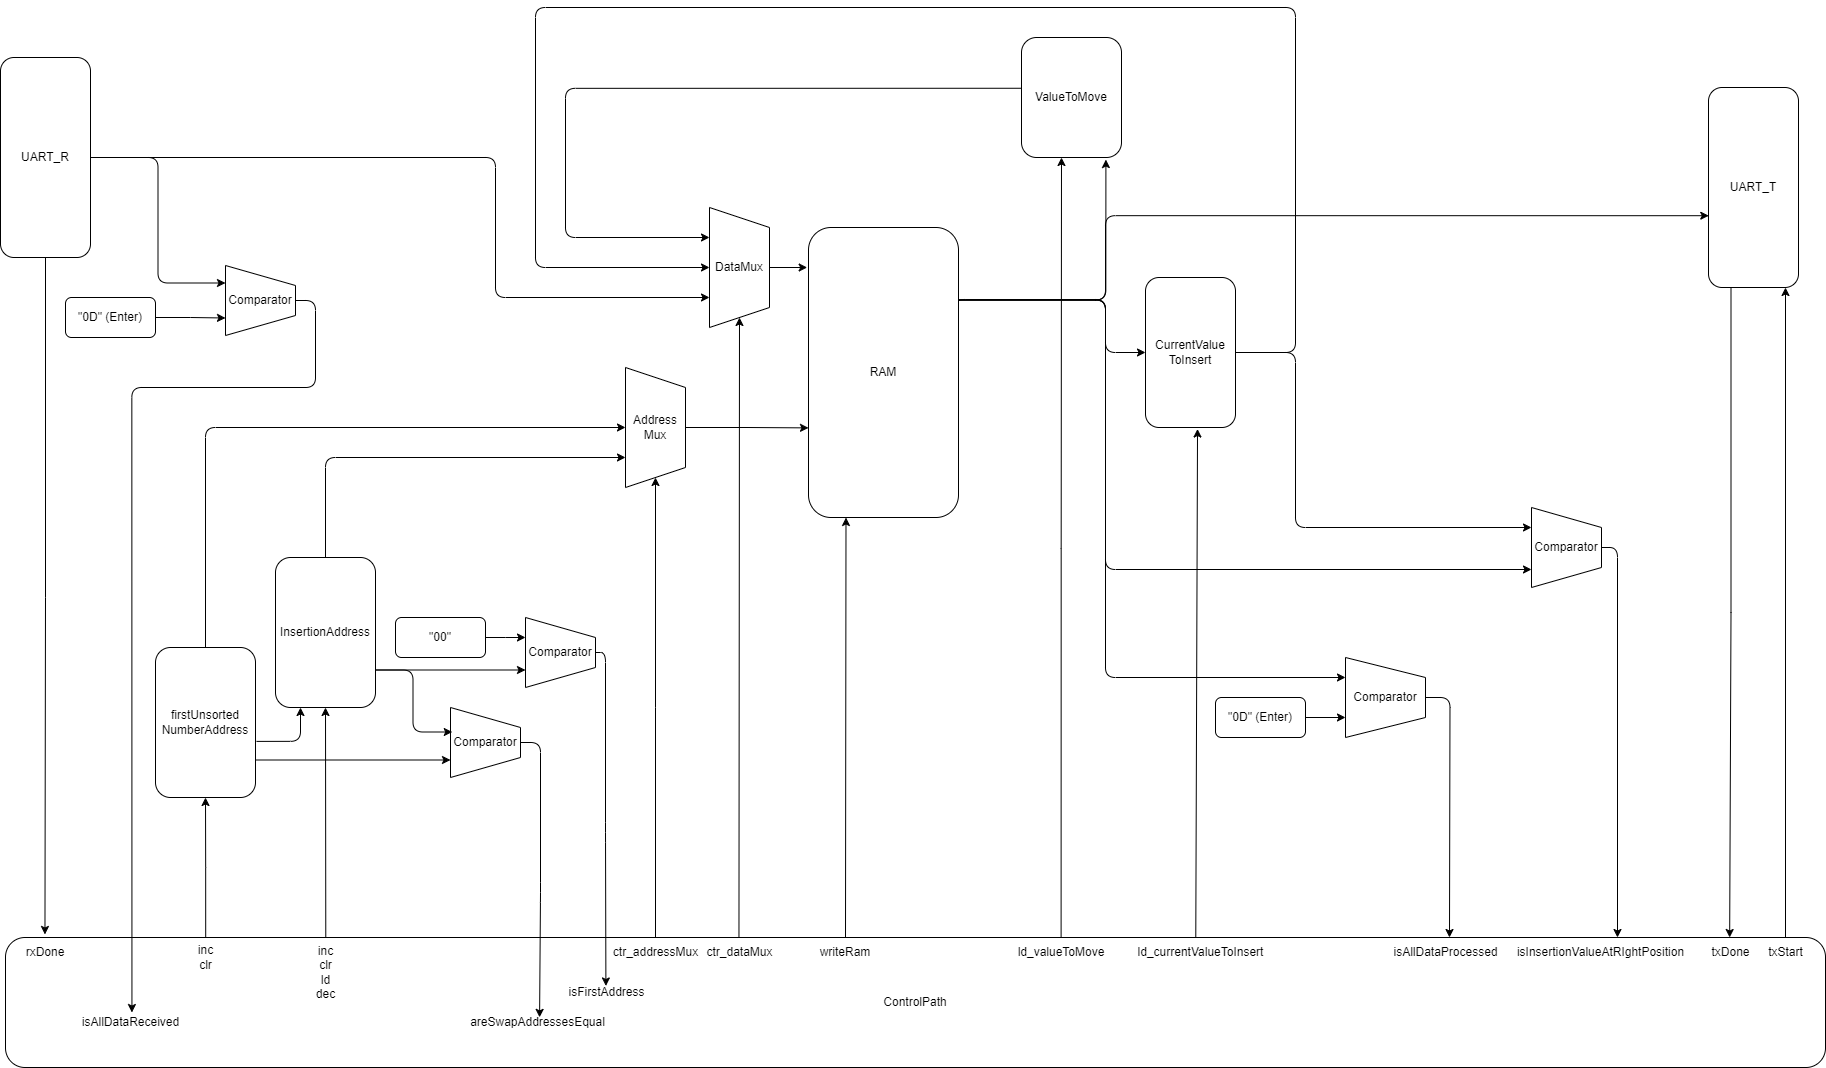
\includegraphics[width=1\linewidth]{Images/FSMDInsertionSort.png}
    \caption{FSMD diagram for the Insertion Sort}\label{fig:fsmd}
\end{figure}
\begin{figure}
    \centering
    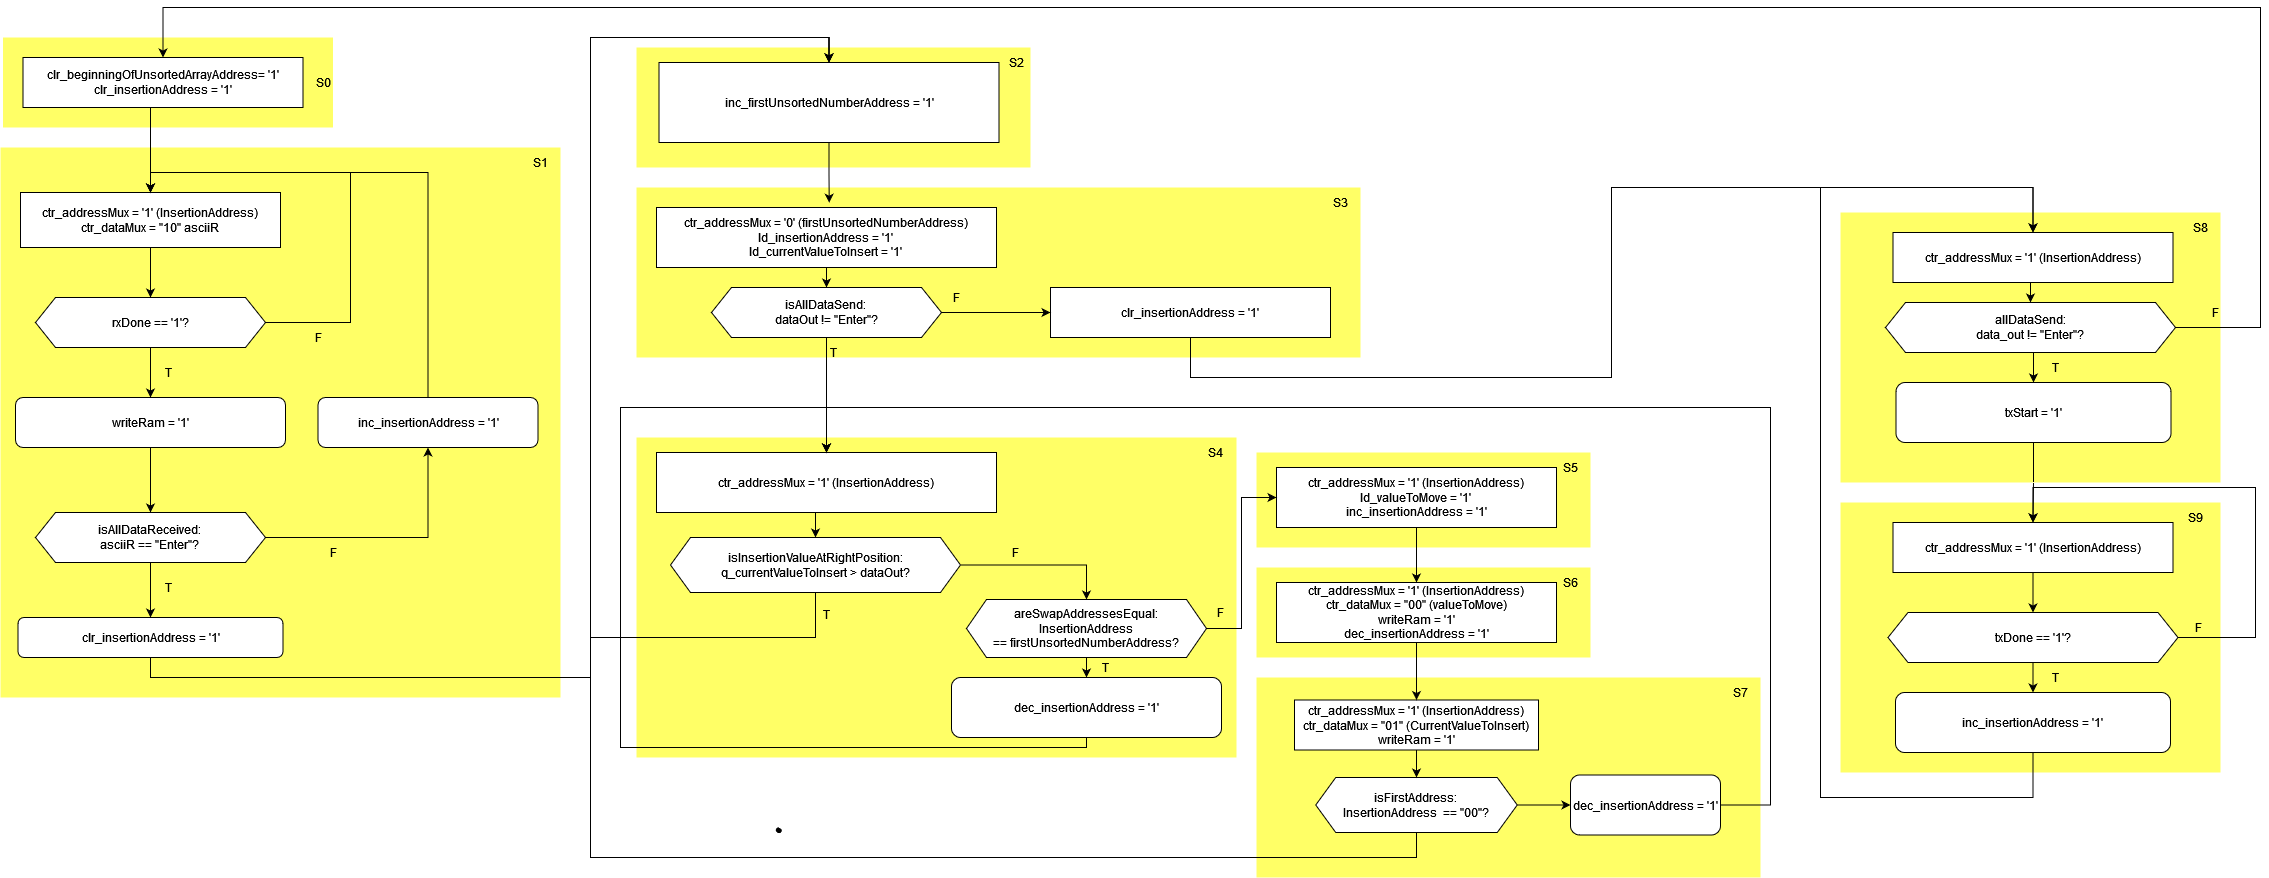
\includegraphics[width=1\linewidth]{Images/ASMDInsertionSort.png}
    \caption{ASMD diagram for the Insertion Sort}\label{fig:asmd}
\end{figure}

\subsection{ASIP}
TODO write in code the mapping of registers to variables in ASMD Chart e.g. Reg[1] = insertionAddress
The second implementation was the application-specific instruction set processor, which we implemented using the ASMD chart. This allowed us to stay consistent with our design choices as well as keep a structred overview of the ASIP implementation. We went through the ASMD chart and converted the boxes into instructions. First we converted the boxes into instructions in natural language. In a second step we converted the natural language into ASIP instructions. We used the one-cycle cpu design as a template for the ASIP design and modified it by changing some core features. This included adding additional components and control signals. The changes which we made, can be seen in \ref{fig:asip} in light blue. The new components are an uart\_rx, uart\_tx for sending and receicing the serial data, a comparator for handling conditional statements and a data-mux since we increased the amount of singals going into the data register. Both of the uart components have a start and a done signal. The comparator only has one output signal which goes trough the control path into the pc\_mux. The data\_mux only needs an input for controlling which data will be forwarded into the data register.\\
Our instruction codes for the ASIP are devided into three logical sections. We go through these sections and explain their idea as well as the reason why we needed additional instructions.\\
The first section (first 8 instructions) handels the receiving of data and writing of data into the data memory. Its starts of by resetting our two main pointers that we use. Next we have a new custom instruction. That instruction is a loop (if the imm value is 0) which loops until uart\_rx send the rx\_done signal. It further send the rx\_start signal to the uart\_rx component and saves the output into the data register. After receiving the data into a register, it is written into the data memory. Next we check if the data, which we just received, is an `Enter'. This would stop the receiving of the data and jump to the next section. This required an additional instruction code. Depending on the result of the comparisson, we either want to jump to a different section or continue with the next instruction. For this we created the comparisson component and connected it to the pc\_mux. Further we created three new instructions: \texttt{Branch if Equal(BEQ)}, \texttt{Branch if Not Equal(BNE)}, and \texttt{Branch if Greater than(BGT)}. We only needed the first instruction for the first section but we implemented all of them at the same time since we knew that we would need the other instructions as well. Since the imm value is used to specify the jump location, the comparisson happens only between two registers.\\
The second section (next 19 instructions) handels the sorting algorithm itself. We load the next value from our not yet sorted area in the array and compare it to an `Enter'. This is to branch to the third section for the output since the `Enter' indicates the end of the array. If the condition is not met, we know that we have a value which needs to be sorted. Next we try to find the position in which the not yet sorted value needs to be inserted. This is done by going from the back to the front until we find a value which is not larger than the new value which we want to insert. Therefore, we needed the new \texttt{BGT} command to do this comparisson. All values along the way are swapped until we find the correct place to insert the unsorted value. The swapping is handeled by instructions $0x12-0x16$. After swapping, we check check if we have reached the first value of the array. This would indicate that we can continue with the next unsorted value. Even though this section might seem to be complex, the logic itself is exactly the same as in the ASMD. Sometimes multiple commands are needed to reflect one box but the branching logic is equal to the ASMD diagram. \\
The last section (last 8 instructions) handels the sending of the data to the uart\_tx. Similar to the other sections, finding an `Enter' value, will branch to the next - in this case first - section. Otherwise we send the next character via serial until we find that `Enter' value. This required two new instructions. One instruction (WR\_UART\_Start) is for starting the uart\_tx component with data from the data memory. The other instruction is a loop which is implemented quite similar to the loop in the first section. This time we loop until we receive the tx\_done signal.\\
The instruction memory had initially space for 32 instructions. We needed more than 32 instructions for our sorting algorithm. Therefore, we extended the instruction memory and all other signals which depend on it by one bit. \\
In the end we have six additional instructions, four additional components, 34 instructions and a couple of changes to the exisiting components and code. The resulting behavior is exactly the same as it is for the FSMD. The code worked on the Basys3 board. This is also achieved by relying heavily on the ASMD diagram for the ASIP design. Further information about the debugging, the implementation complexity and other aspects can be seen following subsections in the second part of the report. \\

\begin{figure}
    \centering
    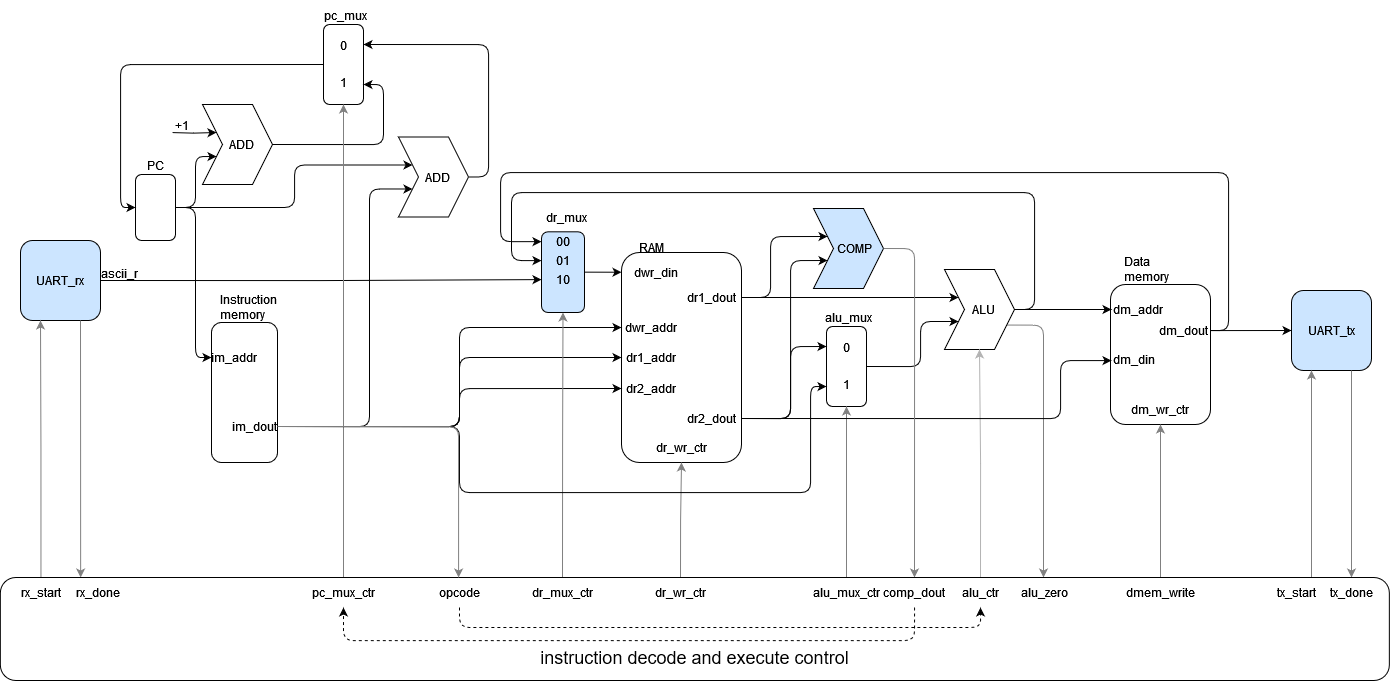
\includegraphics[width=1\linewidth]{Images/ASIP.png}
    \caption{ASIP diagram, based on the same ASIP diagram from the lecture week. The light blue components as well as their connections are new components to enable our Insertion Sort algorithm to be executed.}
    \label{fig:asip}
\end{figure}

\subsection{C coding in Vitis}
Next up, we definied the C program. We setup the project - as we have done it in the lecture week - based on the roadmap of Eric Peronnin. This was done to start on a working version which we could always go back to if and when encoutering errors. This proved to be a valuable resource since the debugger output was at times not explicit when it came to debugging. We started by removing the logic for the LEDs present in the code both in Vitis and afterwards in Vivado by removing the Blocks for the LEDs in the design. We then implemented a basic Insertion Sort algorithm in C from the code examples available in geeksforgeeks\cite{g4g}. Next we changed the input and output behavior. Utilizing the `print' statements for debugging, we managed to get the code working efficiently in a short time span. The majority of time spent on the implementation and debugging mainly revolved around issues with pointers. Since no one in the group had comprehensive experience in C, errors pertaining to pointers and similar issues were to be expected. We verified and tested that our final version of this implementation behaved on the Zybo board exactly the same as the FSMD and ASIP implementation did on the Basys3 board. Once we made sure the code behaved as expected we moved on to the next implementation.

\subsection{Create custom IP block}
Lastly, we implemented the IP block. We expected this to be very similar to the C porgram. As we have do it in the project before, we wanted to start based on some working version. Therefore, we implemted the FIR Filter Project again. \\
We encountered the most issues in this implementation. The first issue we encountered was in the udpating of the platform and application components in Vitis. They seem to have a cache which is not cleared automatically when another component is deleted. So when we made changes in our HLS component, created a new xsa file and updated the platform, we encountered the same behaviour as before. Only deleting the platform and application component in Vitis, fully seemed to clear any cached information. \\
Further, issues were all based on the connection between our application component and our HLS/IP component. As described we started of with the fir filter implementation. Since the fir filter implementation exchanges only single integer values, we wanted to modify it into sending arrays. An array cannot be set as an input for a function, so we used pointers. The values of the pointers were exchanged between these two components. Any further data was not copied. Next, we tried a different angle by exchanging a struct between these two components. The issues with this idea were in the application. We did not manage to find out how to use custom data types with the TODO API library from AMD. We also saw the option that it might be possible to share RAM between these two parts. We opted to switch back to the fir implementation and instead of using an array to exchange the data, we send the data one by one via the existing working exchange of integer values. We managed to build a working version around that idea. After confirming that we have a working version, we refactored the code and finished that part of the implementation. \\
Most of the time for this implementation was spend on the issues that we had. The implementation of the sorting function and the implementation in the end were quite similar to the C-code implementation. We estimate that we spend 75\% of our work in this implementation with dealing with the issues. This can be atributed to the both the lack of knowledge of the tools and libraries as well as a worse debugging experience which explain later in~\ref{sec:debugging} (TODO link to subsection). Due to these issues, we tried a lot of different approaches as well as using ChatGPT (TODO footnote). The solutions from ChatGPT did not prove to be valuable for us. Either it referred us to solution which worked in C but not with the interface between the two components or it created solutions which were overly complicated.

\section{Comparison}
This next section will evaluate the four implementations from different aspects. We chose aspects that should be considered when diciding for a specific implementation. We will conclude with a summary which implementation fits best for which requirement.
\subsection{Design and Implementation Complexity}
In this subsection we want to evaluate how complex it is to design and implement each approach. The FSMD and the ASMD are very close from the design point of view since they rely heavily on each other. In section \autoref{section:fsmd} the design process was already explained for these approaches. Even though the task was not easy we still managed to do it by contibutions of the whole team. The design phase for the FSMD and ASMD took approxemately half a day of work.\\
The implementation of the FSMD and the ASIP varied from each other. Mainly, they differed because of the logic which we used. In FSMD we could use the states that where described in the ASMD. The statements in the ASMD are very close to the final code. While implementing we found out that we had some errors in our design, which could be fixed fast. In total, it took us one and a half day to implement the FSMD.TODO compare with subsection below!\\ 
On the other side, the ASIP implementation needed more abstraction. We converted the states in multiple smaller opcodes, which were developped and then reused multiple times. We needed to figure out the right opcodes, define them the right way and also implement them correctly in our code. This took a little longer than the FSMD. The abstraction was higher, the readability gets more difficult and thus errors where overlooked more easily. Our main source was the lecture and the working code that we implemented while lecture week. All in all, it took us two and a half days to implement the ASIP. TODO compare with subsection below!\\
For the C implementation the designing was rather easy and straight forward. We used our knowledge of the sorting algorithm and the internet to come up with a first draft. For the implementation we used the draft and made small adjustments mainly to include a serial port receiving and transmitting. The C-code design and implementation step was by far the fasted. It only took us one day of work. Obviously, we all had experiance in C coding and that can be one of the reasons why the implementation was done so quickly. \\
Starting the last implementation - the IP Block - we thought of an easy but yet clean design. We wanted to include the already finished C code in the example code of the FIR filter. To do so, we needed to send an whole array - with multiple cells - from the application component to the host component. We did not find a way to do this, reasons for this might be our missing experience in this topic and the lacking documentation on the internet. We came up with other design ideas such as trying to copy the array, creating a self-definied struct or to forward a pointer to the array.\\ 
We implemented all of these ideas and they all run in our C-Simulation and our testbench file. When we were trying to run it with the RTL Simulation, they did no longer work as we expected. Our final design idea was to adapt our C code solution to the code of the aready working FIR-Filter. The design of the implementations took the longest for the IP-Block. We worked roughly four and a half days on the different designs and implementations. We expierienced a lot of different behaviour in the implementaton of the IP-Block. TODO compare with subsection below!\\  
%conclusion:
To conclude, if the design and implementation complexity is a requirement for choosing an implementation we would evaluate the four implementations as follows:
Worst to design and implement is the IP-Block. Here, very specific knowledge is required, and an understanding for the set-up of the application and the host component is needed. Only because an implementation is working within the C-Simulation and the testbench, it will not neccessairy work with the RTL Simulation and on the zybo board. Additionally, the waiting times of the different compiling times, the lack of a good debugging tools (see~\ref{sec:debugging}) and the missing documentation on the internet make the implementation even more difficult.\\
The ASIP is slighly better from a design and implementation point of view: Once the logic of the algorithm is understood the design phase is rather straight forward. For the implementation, a further abstraction step is needed. This can cause problems. Since the opcodes with the register addresses and the immediate values are written in hexadecimal numbers, the readability decreases, so people are prone to overlook errors.\\
The FSMD can help with the problem of readability. Its top file includes all states that were defined earlier in the ASMD. It is easy to compare the ASMD with the code and check if there are any mistakes. So implementation is easier. This is why from a design and implementation point of view FSMD is a decent choice.\\
The best implementation that can be chosen in order for a low design and implementation complexity is the C-Code. A lot of people know basic C programming and there are great documentations on the internet. In contrast to the other solutions AI can help a lot. It can come up with a code, find errors and help with the implementation.\\

\section{Debugging and Verification Complexity}\label{sec:debugging}
The debugging strategies and the complexity of debugging varied greatly in the different implementations. In both the FSMD and the ASIP, we used the simulation in Vivado. In both cases we had to customize the signals that we want to simulate. The difficulty with this debugging lies in finding the first unexpected or abnormal change. In both cases we used both our diagrams to go through the flow and compare our expected values to the simulated values until we found the outlier. This results in two or even three people doing the debugging. Since we worked as a team on this task, this did not present any resource issue. Nevertheless, this form of debugging felt slower and more complicated compared to debugging python code in a modern IDE in which you can mark the line of code, to which you want to jump. Although being a slow process, it still proved to be an effective tool to find any mistakes that we made. We managed to find all our mistakes with this form of debugging. One benefit of this debugging method is that you do not have to know where you want to debug. Since you get many singals at once, the unnormal behaving signal is very likely included. This reduces the amount of restarting the debugging procedure itselfs. \\
For the C-program we used print-statements for debugging. We viewed the output directly via the serial connection in putty. This form of debugging was quite familiar to all team members. It was intiutive and faster compared to the method above, since we did not have to search for the data. However the print-statements have to be included in various places and also have to be deleted afterwards. The code is therefore changed for debugging. Despide this downside we managed to debug quite a bit faster than the first method. \\
Even though the IP block is also code which is written in C, the debugging experience is quite different and more complex than in the method before. Since there are seperated components, the complexity increases and there are more things which can work or not work and need therefore debugging. The building of the HLS component and afterwards the C-simulation could be debugged as normal C-code could be debugged. The difficulties start at the RTL simulation. The RTL simulation could fail without giving good indications of the reasons for it. This could be due to issues in transfering data or because of not sending data or for running into a loop which was not cought in the C-simulation. As far as we could see, there is not even a debugging tool for it. Our solution was to uncomment sections of the code until we find the section which causes the issue. This is complex and prone to errors since the code logic is heavily effected by the debugging. When the RTL simulation worked, it produced a waveform file. However this waveform file was more complex and difficult to understand since there are many signals in the waveform file to represent the logic of the C code. However, the signals are auto generated and therefore have unintuitive names. We tried debugging with this but could not make any use of it. The next point of debugging is in the application component. At this point there are many possible areas in which the bug itself could be located. This means that we can print the values which we send and receive of the HLS component but depending on the results, we cannot located the bug clearly. Due to the lack of knowledge of this interface between the components, we made many mistakes with the interface itself which were neither located in one or the other component and were therefore difficult to debug. \\
The different implementations result in various different debugging experiences and required skills for debugging. We spend the most time for debugging on the last implementation which was unexpected. The complexity of the interaction between the various different parts resulted in a complex debugging process. Further, the lack of tools for debugging this complex situation, resulted in a slow process. \\
%conclusion
All in all the third implementation was by far the fasted to debug. Both the first and the second implementation took some time to debug but it was still manageable. The last implementation was very difficult to debug and it was unpredictable how fast an error could be found. This should be taken into the cost consideration for the implementation.

\subsection{Scalability, Flexibility, Reusability and Maintainability}
The flexibility, adaptability and reusability of the solutions varies a lot. Our first implementation is complementy (TODO what is complementy?) written in VHDL. The FSMD was just specificly designed for this sorting algortihm. There is nothing flexible in this implementation. If we want to change the sorting algorithm, we would have at least to redesign the full control flow. Depending on the sorting algorithm, we might need more additional components. Everthing has likely to be renamed and restructured. At that point a new algorithm would effect anything in the code but the most basic components. Any other algorithm besides sorting algorithms would likely change the code completely. Anything which is already implemented in hardware has to be changed fully or is not reusable. \\
The ASIP implementation is a little bit more flexible. A change in sorting algorithms changes the control flow. However it depends on the sorting algorithm if anything else needs to be changed. Since the instruction set can be reused for anything, similar algorithms can also be run on the ASIP. Just the instruction RAM needs to be exchanged. This enables small changes even after the hardware is created. However the complexity of implementing a change is rather high. It is not easy predictable what consequences a single new instruction can have on all other instructions. \\
The fourth implementation is more flexible than the first two implementation. The huge flexibility benefit comes the fact that is it not specified how the IP blocks are used. The IP blocks act as predefined algorithms which are likely to be used and optimised. What data and how the data flows into these algorithms, is not specified at the time of creating the hardware. Since there are many algorithms for different standards, this concept can be seen in many modern computers and chips. Standard algorithms for video encoding and deconding can be implemented directly into the hardware. Other algorithms for hashing or encryption/decryption of messages can also be implemented in hardware to increase the speed of opertaion. Any mistakes in the implementation of the IPs, can however still result in high costs and broken products if this is not detected before creating the hardware. \\
The third implementation is the most flexible implementation. In this implementation there is nothing specific about the hardware. The code can be deployed to any hardware which can run the C code. Any mistakes in the code can be fixed by redeploying the code to the hardware. Any new algorithms can also be deployed, additional functionality can be added afterwards and maintaining it is possible as long as the hardware does not break. This makes it undoubtfully the most flexible implementation. However at this point we lose the benefits of implementing algorithms in hardware. \\
The solutions one, two and four offer different kinds of flexibility. Depending on the clarity of requirements and the maintainability it might not be possible to chose the first or second implementation. Therefore, implementing a few crucial algorithms as IP blocks, might be the middle ground which is chosen to ensure that there is still enough that can be changed after deployment. If even that is not possible, the only solution that remains is writing non hardware specific code.

\subsection{Other comparing methods}
EFFICIENCY:\\
The following paragraph will analyze the efficiency of the approaches from various perspectives including execution speed, power consumption, and resource utilization. Since we are using two different hardware bords we do not want to compare the values we get for the execution speed, power consuption and the resource utilization. Due to the different hardware the platform for a just comparision is not given. In the next section we will thus concentrate on the theory behind our implementations.\\
FSMD designs offer the highest level of efficiency in terms of execution speed and power consumption for fixed, predefined algorithms such as Insertion Sort. In FSMD, the algorithm is hardwired into a finite state machine with a dedicated data path, allowing for highly optimized data flow and minimal control overhead. As a result, FSMD can execute the Insertion Sort algorithm in a very short time, often approaching the theoretical minimum number of cycles for the given hardware.In terms of power efficiency, FSMD is typically superior due to its simple and optimized control logic, which minimizes switching activity and dynamic power consumption.\\
ASIP designs strike a balance between flexibility and efficiency. While ASIPs are not as efficient as FSMD in terms of execution speed and power consumption, they offer significant flexibility due to their programmability. The Insertion Sort algorithm can be efficiently implemented using a custom instruction set, which allows for hardware-level optimizations specific to sorting tasks. ASIPs can also leverage parallelism and pipelining techniques to enhance their efficiency, making them suitable for applications that require moderate performance with the flexibility to handle a variety of tasks.\\
The C implementation of Insertion Sort, running on a general-purpose processor, offers the lowest efficiency among the compared approaches. Since general-purpose processors are not optimized for specific tasks like sorting, execution is slower, and power consumption is higher compared to specialized hardware implementations. The control flow of the Insertion Sort algorithm in C involves multiple levels of abstraction (such as instruction decoding and memory accesses), which leads to additional overhead.\\
A custom IP block synthesized using HLS is designed to achieve high efficiency with less design effort compared to FSMD. By describing the algorithm in a high-level language (such as C or C++), HLS tools automatically generate hardware that is optimized for the target algorithm, including Insertion Sort. This allows for more efficient use of resources than ASIP while offering some flexibility through design-level changes. Custom IP blocks can take advantage of architectural optimizations such as pipelining, data-level parallelism, and reduced memory access, leading to improvements in execution speed and power consumption. This approach is ideal for applications that need efficient hardware but also require rapid development cycles.\\
%conclusion
The most efficient approach depends on the application context. For maximum performance and minimal power consumption, FSMD is ideal. ASIP and custom IP blocks offer a good trade-off between flexibility and efficiency. From these aspects the C implementation is rated the least best.
\\
CONCURRENCY:
\section{Concurrency Comparison of FSMD, ASIP, Custom IP Block, and C Implementations}
In this next section we want to compare our four implementations under the aspect of concurrency. This requirement refers to the ability of a system to execute multiple operations or tasks simultaneously.\\
FSMD is inherently limited in its concurrency capabilities. The finite state machine is designed for sequential control flow, with operations occurring in a fixed order as determined by the state transitions. Although FSMD can achieve high efficiency for specific tasks, it is typically constrained to executing one operation at a time. This lack of parallelism makes it less suited for applications requiring high degrees of concurrency. While multiple instances of FSMD could theoretically run in parallel, this approach introduces significant hardware complexity, which may not be cost-effective.\\
ASIP designs offer more opportunities for concurrency compared to FSMD. By incorporating custom instructions that exploit parallelism, ASIPs can perform multiple tasks simultaneously, such as executing multiple data operations or processing several instructions in parallel.\\
Custom IP blocks synthesized using High-Level Synthesis (HLS) can achieve high levels of concurrency by exploiting hardware-level parallelism. HLS tools allow designers to specify parallel execution of multiple operations at the algorithmic level, which can then be translated into parallel hardware structures. This makes custom IP blocks highly efficient in terms of concurrency, particularly when sorting large datasets where parallel operations can significantly reduce execution time.\\
C implementations running on general-purpose processors, benefit from modern CPU features such as multi-threading and hardware-level concurrency support. General-purpose processors can take advantage of multiple cores to perform parallel sorting tasks, provided the algorithm is written in a way that supports concurrency. Optimizations such as parallel execution of sub-tasks or using concurrency frameworks can improve performance, but the scalability is limited compared to specialized hardware solutions like ASIP or custom IP blocks.\\
%conclusion
To conclude, custom IP blocks offer the highest level of concurrency, followed by ASIP, which provides moderate parallelism through custom instruction sets. C implementations can accomplish concurrency through different threads, but they efficiency is not as high as the ASIP. Lastly, FSMD implementations remain largely sequential and are thus rated worst from a concurrency perspective.\\

\section{Scalability Comparison of FSMD, ASIP, Custom IP Block, and C Implementations}
SCALABILITY:
The scalability of each implementation varies quite heavily depending on the a couple factors. First is the complexity of the design. The design complexity in the context of scalability focuses on how many components are connected to one another and dependant on each other. Flexability is quite important in this regard as good Flexability will often lead to good scalability. Scalability is also reduced if the logic behind each implementation is also difficult to adapt to other applications. In this regard FSMD systems perform worse than our other implementations. It is a far less versatile system to adapt into multiple applications due to its tightly-coupled nature, where the data path and control path are specifically tailored for a particular task. This means the FSMD needs to undergo significant restructuring if we wish to upscale it.\\
The scalability of the ASIP implementation is a lot higher compared to our FSMD design. This is because the flexibility that the ASIP design provides us with. The ASIP design enables us to add new instructions or modify them without needing to change the core structure of the processor a lot. A key aspect of scalability in the ASIP implementation is the expansion we were able to make to the instruction memory from 32 maximum instructions to 64 instructions. We did this to accommodate the additional operations required. The lack of difficulty in which it took to expand the instruction memory demonstrates how the ASIP can be scaled to handle more complex algorithms with larger instruction sets. Since we are able to expand the ASIP implementation to accomodate for more complex tasks it means that the adaptability is quite a lot better than the FSMD which requires a lot of logical refactoring to become optimal with a new design.\\
The C-code implementation was quite simple as minor adjustsments would be needed to scale up this implementation. If this implementation were to be mass produced then simply acquiring the required hardware is the costly part of scaling up this implementation. The IP block implementation is quite difficult to determine how scalable it is. Once the system is understood and a working implementation has been reached, it would be possible to scale it up. In practice however the debugging and error checking so complex at times that trying to scale up production for this implementation would be a daunting task. 

\subsection{Production Cost}
In this next paragraph we want to dive deep into the production cost of each approach. We will focus mainly on the hardware production costs which will include the non-recurrent costs (NRC) and the per-unit costs. NRE costs refer to one-time expenses incurred during design and development, while per-unit costs account for expenses related to manufacturing each individual unit of the hardware or software. Since we only used the development boards which are not used in a final product the following paragraph contains mainly theory that is referred to our project.\\
The FSMD approach involves designing a specialized hardware circuit for the Insertion Sort algorithm. FSMD designs typically require substantial NRE costs because of the need for specialized hardware tailored specifically to the Insertion Sort algorithm. After design verification, the physical fabrication of FSMD on silicon chips involves high initial costs, particularly for smaller production volumes. The cost per unit decreases with large-scale production but remains high due to the dedicated hardware architecture. For general use cases, the initial design and fabrication costs present significant barriers.\\
ASIP-based designs strike a balance between custom hardware (like FSMD) and general-purpose processors (like the C implementation). ASIPs are programmable but tailored to a specific application domain, such as sorting algorithms. The per-unit production cost is generally lower than that of FSMD because ASIPs leverage partially standardized fabrication processes. However, these costs increase when ASIPs require customization beyond standard architectures. The NRC costs are moderate since common processor componenst can be used. This is also the reason why we have moderate per-unit costs.\\
The C implementation of Insertion Sort runs on general-purpose processors with a standard instruction set architecture (ISA). It requires no specialized hardware. The cost structure for C implementations is radically different from hardware-based solutions like FSMD and ASIP. The NRE costs for C implementations are minimal, as they require no custom hardware design. Since C implementations run on off-the-shelf hardware, the per-unit production cost is negligible. 
%The same general-purpose processor can run a variety of applications, including Insertion Sort, which leads to extremely high economies of scale in production. Both the NRC and the per-unit costs are low to very low. 
While the C implementation offers the lowest production costs, it sacrifices performance and power efficiency compared to FSMD and ASIP. Therefore, it is best suited for general-purpose applications where cost is a primary concern and performance can be compromised.\\
A custom IP block is developed using High-Level Synthesis (HLS), where a high-level language like C or C++ is used to define the algorithm, and the design is synthesized into hardware. This approach provides the flexibility of software design with the performance benefits of hardware.The NRE costs for custom IP blocks using HLS are lower than those for FSMD because HLS allows for the automatic generation of hardware from high-level descriptions. This reduces the manual effort required in hardware design, cutting down verification time and labor costs. The per-unit production cost for custom IP blocks is similar to FSMD since the synthesized hardware still needs to be fabricated on silicon. However, the flexibility in design allows for optimization, potentially reducing chip area and power consumption, which can lower per-unit costs. The custom IP block approach strikes a balance between development effort and hardware efficiency. While the NRE costs are higher than for a pure software solution, they are lower than FSMD and ASIP.
%conclusion
The production costs of FSMD, ASIP, custom IP blocks using HLS, and C implementations of the Insertion Sort algorithm differ significantly. FSMD incurs the highest costs due to the custom hardware design and fabrication, making it suitable for specialized, high-performance applications. ASIP offers more flexibility with moderate production costs, while custom IP blocks using HLS provide an efficient trade-off between flexibility and hardware performance. Finally, the C implementation is the most cost-effective for general-purpose hardware, with minimal development and production costs but lower performance. 

\subsection{Development Cost}
This section aims to quantify the amount of time that we spend on each implementation and thereby give an estimation how the cost of the different implementations can vary. All three of us worked on all implementations at the same time. To reduce the complexity, the time we spend on each implementation is only given as it would be for one person. If we for example spend one day working on an implementation, this would be noted as 8h even though three people worked on it for eight hours which would result in the actual time of 24h. This is done since we want to focus on the relative development cost between the solutions instead of the actual development cost.\\
For the FSMD development, we spend around 23h. This includes the time for the diagram, code refactoring and debugging until the implementation worked. Even though we cannot quantify it, we spend a significant amount of time on the initial design. We created both the FSMD and the ASMD diagrams first and this took around 6-8h. The second day was mainly spend on implementation and it ended in first tests and debugging. The rest of the hours were spend on refactoring, smaller improvements and get every edge case working without any issues. This implementation had a steady progress throughout the whole time.\\
For the ASIP development, we spend around 20h. Since we used the ASMD diagram heavily for this, we did not have to develop any new logic. This contributed to the ASIP implementation taking less time than the FSMD implementation. It was unexpected to us. We thought the ASIP implementation would take around 10\%-30\% more time compared to the FSMD implementation instead of this being the other way around. During the ASIP implementation, we spend around the first 10h-12h on creating the logic and chaging the existing processor. The last 6h-8h were used for debugging and refactoring. It also helped that we already debugged the FSMD first. We were more trained on the debugging process and we had little to debug. \\
% TODO: do we want to write number up tp 12 as words?
For the C-Code implementation it took us about 7,5h to do the full implementation and getting the code to run on the Zybo board. Most of the time for this implementation was spent on setting up Vitis and debugging issues with pointers. Since we took an implementation from a reputable source, we spend little to no time on the algorithm itself. None of us has programmed a lot in C and therefore, we made some mistakes in the pointer handling.\\
For the C-Code implementation with the IP block, it took us around 21,5h to get a working version. We spend around 4-6h on the actual coding and most of the time with debugging. This was completely due to the lack of understanding of the software and the connection between the software and hardware component. We underestimated both the complexity of this task as well as the time that we are going to spend on this implementation. The progress with this implementation was far from linear. 6h before finishing the implementation we still were unsure about the logic and the algorithms for receiving, sending and transferring between the different components. This uncertainty should not be underestimated. The lack of knowledge caused considerable delay in this implementation. \\
% also include the long and many compiling time here? It took us about half an hour to build a HLS component, didn't it?
We had three implementation which roughly took the same amount of time and one implementation with roughly a third of the time. The short implementation was done purely in software while all other implementations had at least a hardware component. This shows that the development costs are considerably higher for hardware implementations compared to pure software implementation. We expected to have a larger time difference in the implementation time between the different hardware implementations. Our project task was likely not complex enough to differentiate in fine detail between the implementation cost for the different hardware implementations.

\section*{Acknowledgment}

We confirm that there was no significant difference in the contribution to the work.

\printbibliography

\begin{appendices}
\section{Use of AI}
used for write production cost section promt: Please write a one page scientific latex report as a professor of Computer science. The topic is the cost comparison between the production of FSMD, ASIP and a C implementation of a Insertion Sort algorithm. Please use a scientific writing style and include all sources that were used. Remember to write your report in latex code.
\end{appendices}

\end{document}
